\documentclass[]{scrreprt}
%\usepackage{amsmath,amsfonts,graphicx}
%\usepackage{multirow}
%\usepackage{pslatex}
%\usepackage{tabularx}
%\usepackage{comment}
%\usepackage{xspace}
%\usepackage{array}
\usepackage{caption}

\RequirePackage{fix-cm}
\usepackage{graphicx}
\usepackage{color,soul}
\usepackage{todonotes}
\usepackage{subfigure}
\usepackage{amsmath}
\usepackage{empheq}
\usepackage{mathrsfs}
\usepackage{natbib}
\usepackage{listings}
\usepackage{rotating}
\usepackage{hyperref}
\usepackage{epstopdf}


\DeclareCaptionFont{white}{\color{white}}
\DeclareCaptionFormat{listing}{\colorbox{gray}{\parbox{\textwidth}{#1#2#3}}}

\graphicspath{
{figures/}
}

\newcommand{\uo}{\mbox{UO\textsubscript{2}}\xspace}

\setcounter{secnumdepth}{3}

\newcommand{\moose}{{MOOSE}}
\newcommand{\redback}{{REDBACK}}
\newcommand{\pd}{\ensuremath{\partial}}
\newcommand{\pdiff}[2]{\ensuremath{\pd_{#2} #1}}
\newcommand*\widefbox[1]{\fbox{\hspace{1em}#1\hspace{1em}}}


\begin{document}


\title{Redback Theory Manual}
\author{Thomas Poulet \\ CSIRO 
	\and Manolis Veveakis \\ UNSW}
\maketitle

\tableofcontents

%%%
\chapter{Introduction}

The \redback{} application was developed to model multi-physics \textit{Rock mEchanics with
Dissipative feedBACKs} in a tightly coupled manner. It is based on the Multi-physics Object Oriented Simulation Environment \moose{}\footnote{http://mooseframework.org} \citep{Gaston2009} which proposes a powerful and flexible platform to solve multi-physics problems implicitly and in a tightly coupled manner on unstructured meshes. \moose{} aims at providing a wide range of modules to model various physical phenomena, including rock mechanics, which are as flexible as possible and can be easily coupled together. By comparison, \redback{} is  
The philosophy behind \redback{} is to focus on a non-dimensional formulation of the problem in order to focus on the physical processes at play

Please cite...


\chapter{Governing equations}
\label{chapter:gov_eqs}



The system in its final form is
\begin{subequations}
\label{eq:final_system_of_equations_dimensionless}
\begin{empheq}[box=\widefbox]{align}
  0 &= \pdiff{\sigma^{\prime}_{ij}}{j} + \pdiff{p_f}{i} + b_i, \\   
  0 &= \pdiff{p_f}{t} + Pe\: v^p_i \pdiff{p_f}{i} -
  Pe\:v^T_i \pdiff{T}{i} - \pdiff{\left[\frac{1}{Le} \pdiff{
  p_f}{i} \right]}{i} \\ \nonumber
  ~ & \qquad\qquad - \Lambda \pdiff{T}{t} +
  \frac{Pe\:\dot{\epsilon_V}}{\bar{\beta}\:\sigma_{ref}} -\frac{1}{Le_{chem}}
  \omega_F, \\
  0 &= \pdiff{T}{t} + Pe\:\bar{v_i}\pdiff{T}{i} - \pd_{ii}^2 T - Gr
  \: \sigma_{ij}^{pl}\dot{\epsilon}_{ij}^{\,pl}  \\ \nonumber
  ~ & \qquad\qquad + Da_{endo}\: (1 - s)(1 - \phi)e^{\frac{Ar_F\:\delta T}{1+\delta T}} \\ \nonumber
  ~ & \qquad\qquad - Da_{exo}\:\: s  (1 - \phi)\Delta \phi_{chem} e^{\frac{Ar_R\:\delta T}{1+\delta T}}.
\end{empheq}
\end{subequations}

All dimensionless groups are defined in Tab.~\ref{tab:dimensionless_nbs} and
\begin{align*}
  \bar{\beta} &= (1-\phi)\beta_s + \phi\beta_f, \\
  v_i^p &= (1-\phi)\frac{\beta_s}{\bar{\beta}} v_i^s + 
    \phi\frac{\beta_f}{\bar{\beta}}v_i^f, \\
  v^T_i &= (1-\phi)\frac{\bar{\lambda}_s}{\bar{\beta}} v_i^s + 
    \phi\frac{\bar{\lambda}_f}{\bar{\beta}} v_i^f,\\
  \bar{v_i} &= \frac{\rho_s}{\bar{\rho}} v_i^s + \frac{\rho_f}{\bar{\rho}} v_i^f, \\
  \omega_F &= (1-\phi)(1-s)\exp\left(\frac{Ar_F \: \delta T}{1 + \delta T}
  \right), \\
  \omega_R &= (1-\phi)\:s\:\Delta \phi_{chem}\exp\left(\frac{Ar_R \: \delta
  T}{1 + \delta T} \right), \\
  \dot{\epsilon}^{pl}_{ij} &= \dot \epsilon_0 \: \exp\left( \frac{Ar \: \delta
  T}{1 + \delta T}\right) \sqrt{ \left\langle\frac{q -
  q_Y}{\sigma_{ref}}\right\rangle^{2m} + \left\langle\frac{p
  - p_Y}{\sigma_{ref}}\right\rangle^{2m}} \frac{\partial f}{\partial
    \sigma_{ij}}.
\end{align*}



The total porosity $\phi$ is expressed as the sum of its initial value, $\phi_0$,
and the newly created interconnected pore volume. Pore volume can be created
by mechanical ($\Delta\phi_{mech}$) and chemical ($\Delta \phi_{chem}$)
processes such that the total porosity reads
\begin{eqnarray}
    \label{eq:porosity}
    \phi = \phi_0 + \Delta\phi_{mech} + \Delta\phi_{chem} = \frac{V_{B}}{V},
\end{eqnarray}
where $V_B$ is the volume occupied by fluid $B$.  The evolution of mechanical
porosity contains two components, a plastic part $\Delta
\phi^{pl}_{mech}=\epsilon^{pl}_V$, with $\epsilon^{pl}_V$ the volumetric plastic strain, and an
elastic one $\Delta \phi^{e}_{mech}=(1-\phi)\left( \beta_s \Delta p_f -
\lambda_s \Delta T \right)$
where $\beta_s$ and $\lambda_s$ are compressibility and
thermal expansion coefficients of the solid phase, respectively.

\section{Rescaling}
\label{sec:rescaling}
A particularity of \redback{} is to work with dimensionless parameters, in line with the purpose of studying system stabilities. As such, the variables used in the final system of equation (Eq.~\ref{eq:final_system_of_equations_dimensionless}) are all dimensionless and defined as such:
\begin{subequations}
  \label{eq:dimensionless_defs}
  \begin{align}
  p^* &= \frac{p_f}{\sigma_{ref}}, \\   
  T^* &= \frac{T-T_{ref}}{\delta T_{ref}}, \\   
  x^* &= \frac{x}{x_{ref}}, \\   
  t^* &= \frac{c_{th}}{x^2_{ref}}t, \\   
  V^* &= \frac{V}{V_{ref}}.
  \end{align}
\end{subequations}
with $c_{th} = \alpha / (\rho C_p)_m$. The derivations of those dimensionless variables is detailed in Sec.~\ref{chapter:derivations}.

Note that the time can in turn be rescaled a second time for numerical reasons (see Sec.~\ref{subsec:time_rescaling}).


\section{Chemical damage}
\label{sec:chem_damage}

Thermally activated chemical reactions are allowed to take place and
in this work we concentrate on (de-)hydration reactions of the form
\begin{equation}
  \label{eq:reaction}
  \nu_1 AB_{s} 
  \overset{\omega_F}{\underset{\omega_R}{\rightleftharpoons}} \nu_2 A_{s} + \nu_3 B_{f},
\end{equation} 
where the subscripts $s$ and $f$ refer to solid and fluid phases and $\nu_i$
$(i=1,2,3)$ are stoichiometric coefficients.  The reaction
equation~\eqref{eq:reaction} states that the solid $A$ can release/bind the
component $B$ into/from the fluid phase which increases/reduces the pore pressure.

The kinetics of the decomposition reaction~\eqref{eq:reaction} are assumed
to follow a standard Arrhenius dependency on temperature 
\citep{Poulet2014}. As a result, the rates of the forward, $\omega_F$, and
reverse reaction, $\omega_R$ (let $\nu_1=\nu_2=\nu_3=1$) can
be expressed as \citep{Alevizos2014}
\begin{subequations}
\label{eq:reaction_rates_txt}
\begin{align}
  \omega_F &=  \frac{\rho_{AB}}{M_{AB}} (1 - \phi)(1 - s)  k_F e^{-Q_F/RT}, \\
  \omega_R &=  \frac{\rho_{A} \rho_{B}}{M_A M_B} (1 - \phi) s \Delta\phi_{chem}
  k_R e^{-Q_R/RT},
\end{align}
\end{subequations}
where $\rho_i$ and $M_i$ $(i = A, B, AB)$ are the densities and molar masses of
the respective constituent,
$k_F,k_R$, $Q_F,Q_R$ are the pre-exponential factors and activation enthalpies
of the forward and reverse reaction,
$\phi$ is porosity and $\Delta\phi_{chem}$ denotes change in porosity due to 
chemical processes. We define the solid ratio
\begin{eqnarray}
    \label{eq:s}
    s = \frac{V_{A}}{V_s} = \frac{V_{A}}{(1-\phi) V},
\end{eqnarray}
where $V$ is a representative volume, $V_A$ and $V_s$ is the volume of solid
phase $A$ and all solid within $V$, respectively. The solid ratio is a measure
of the extend of reaction~\eqref{eq:reaction}. Subsequently, the total
reaction rate is
\begin{equation}
 \label{eq:reaction_rate_total}
\omega = \left[(1 - s) - s  \Delta \phi_{chem} \frac{\rho_{A}
\rho_{B}}{\rho^2_{AB}} \frac{M^2_{AB}}{M_A M_B} K^{-1}_c e^{\Delta h/RT}
\right] (1 - \phi) \frac{\rho_{AB}}{M_{AB}} k_F e^{-Q_F/RT}
\end{equation}
where $K_c = k_F/k_R$ and $\Delta h = Q_R - Q_F$.  The expressions for the
dependency of the porosity $\phi$ and solid ratio $s$ on the reaction kinetics
are described in detail in \cite{Alevizos2014} and briefly summarized here.

We assume the following relations for the partial molar reaction rates of the
species involved
\begin{subequations}
\label{eq:js}
\begin{align}
  \omega_{AB} &= - \left[ \frac{\rho_{AB}}{M_{AB}} (1 - \phi)(1 - s)
  \right]^{\nu_1} k_F \exp(-Q_F/RT), \\
  \omega_A &= \left[ \frac{\rho_{A}}{M_A} (1 - \phi) s \right]^{\nu_2} k_A \exp(-Q_R/RT), \\
  \omega_B &= \left[ \Delta\phi_{chem} \frac{\rho_{B}}{M_B} \right]^{\nu_3} k_B
  \exp(-Q_R/RT),
\end{align}
\end{subequations}
and those rates are linked by the stoichiometry of the considered reaction~\eqref{eq:reaction} as
\begin{equation}
  \label{eq:j_equal}
	-\frac{\omega_{AB}}{\nu_1} = \frac{\omega_A}{\nu_2} = \frac{\omega_B}{\nu_3}.
\end{equation}
From Eqs.~(\ref{eq:js}-\ref{eq:j_equal}) and for $\nu_1=\nu_2=\nu_3=1$ we
derive the poro-chemical model
\begin{subequations}
\label{eq:s_phi_chem}
\begin{align}
  \Delta \phi_{chem} &= A_{\phi} \frac{1-\phi_0}{1 + \frac{\rho_{B}}{\rho_{A}} \frac{M_{A}}{M_{B}} \frac{1}{s}}, \\
  s &= \frac {\omega_{rel}} {1+\omega_{rel}},\\
  \omega_{rel} &= \frac{\rho_{AB}}{\rho_{A}} \frac{M_{A}}{M_{AB}} K_c \exp
  \left( \frac{\Delta h}{RT} \right),
\end{align}
\end{subequations}
where
$A_{\phi}$ is a coefficient that determines the amount of the
interconnected pore-volume (porosity) created due to the reaction. We assume
that all the fluid generated contributes to the interconnected pore volume, and
thus set $A_{\phi} = 1$.




\begin{table}
  \todo[inline]{Damkohler numbers to check}
  \caption{Dimensionless parameters used in \redback{}. The coefficient $\delta$ is defined
such that $T^{\star} = (T-T_{ref})/(\delta T_{ref})$}
\label{tab:dimensionless_nbs}
\begin{tabular}{@{} l p{0.18\textwidth} l p{0.52\textwidth} @{}}
\hline\noalign{\smallskip}
Group & Name & Definition & Interpretation \\
\noalign{\smallskip}\hline\noalign{\smallskip}
$Gr$ & Gruntfest number & $\frac{\chi\sigma_{ref}\dot{\epsilon}_{ref} x^2_{ref}}{\alpha \delta T_{ref}}$ & ratio of mechanical rate converted into heat over rate of diffusive processes \\
$Da_{endo}$ & Endothermic Damk\"{o}hler number & $\frac{A_{endo} h_{endo} \rho_{AB} x^2_{ref}}{\alpha \delta T_{ref}}$ & ratio of endothermic reaction rate over rate of diffusive processes \\
$Da_{exo}$ & Exothermic Damk\"{o}hler number & $\frac{A_{exo} h_{exo} \rho_{AB} x^2_{ref}}{\alpha \delta T_{ref}}$ & ratio of exothermic reaction rate over rate of diffusive processes \\
$Ar$ & Arrhenius number & $Q_{mech}/(R T_{ref})$ & Ratio of activation energy over thermal energy \\
$Ar_F$ & Forward Arrhenius number & $Q_F/(R T_{ref})$ & Ratio of activation energy of forward reaction over thermal energy \\
$Ar_R$ & Reverse Arrhenius number & $Q_R/(R T_{ref})$ & Ratio of activation energy of reverse activation energy over thermal energy \\
$Le$ & Lewis number & $c_{th}/c_{hy}=\frac{\mu_f\:c_{th}\:\beta^*_m}{k \: \sigma_{ref}}$ & Ratio of thermal over mass diffusivities \\
$Le_{chem}$ & Chemical Lewis number & $\frac{c_{th}\sigma_{ref}\beta_m }{x^2_{ref} A_{endo}}\frac{\rho_{B}}{\rho_{AB}} \frac{M_{AB}}{M_{B}} \left( \frac{\rho_B}{\rho_f} - \frac{\rho_B}{\rho_s}\right)e^{-Ar_F}$ & Ratio of thermal over chemical diffusivity of forward reaction \\
$\bar{\Lambda}$ & Thermal pressurisation coefficient & $\frac{\lambda_m}{\beta_m}\frac{\delta \:T_{ref}}{\sigma_{ref}}$ & Normalised thermal pressurisation coefficient, with $\lambda_m$ and $\beta_m$ the mixture thermal expansion and compressibility \\
$Pe$ & P\'{e}clet number & $x_{ref}V_{ref}/c_{th}$ & Ratio of temperature advection rate over diffusion rate \\
\noalign{\smallskip}\hline
\end{tabular}
\end{table}


\chapter{Code architecture}
\label{chapter:code}
\section{Kernels}
Here is the list of all kernels implemented in \redback{} to solve the system of Eq.~\ref{eq:final_system_of_equations_dimensionless}:
\begin{align*}
  \\ \\ 
  0 &= \overbrace{ \pdiff{\sigma^{\prime}_{ij}}{j} + \pdiff{p_f}{i} + b_i }^{\begin{rotate}{10}RedbackStressDivergenceTensor\end{rotate}} , \\ 
  \\   
  0 &= \overbrace{ \pdiff{p_f}{t} }^{\begin{rotate}{15}TimeDerivative\end{rotate}} 
       + \overbrace{ Pe\: v^p_i \pdiff{p_f}{i}
       - Pe\:v^T_i \pdiff{T}{i} }^{\begin{rotate}{15}RedbackMassConvection\end{rotate}} 
       - \overbrace{ \pdiff{\left[\frac{1}{Le} \pdiff{p_f}{i} \right]}{i} }^{\begin{rotate}{15}RedbackMassDiffusion\end{rotate}} 
       \\ \nonumber
  ~ & \qquad 
  - \underbrace{ \Lambda \pdiff{T}{t} }_{\begin{rotate}{-15}RedbackThermalPressurization\end{rotate}} 
  \qquad\quad+ \qquad \underbrace{ \frac{Pe\:\dot{\epsilon_V}}{\bar{\beta}\:\sigma_{ref}}  }_{\begin{rotate}{-15}RedbackPoromechanics\end{rotate}} 
  \: - \: \underbrace{ \frac{1}{Le_{chem}}  }_{\begin{rotate}{-15}RedbackChemPressure\end{rotate}} 
  \omega_F, \\ \\ \\
  0 &= \underbrace{ \pdiff{T}{t}   }_{\begin{rotate}{-25}TimeDerivative\end{rotate}} 
  +  \underbrace{ Pe\:\bar{v_i}\pdiff{T}{i}   }_{\begin{rotate}{-25}RedbackThermalConvection\end{rotate}} 
  - \underbrace{ \pd_{ii}^2 T   }_{\begin{rotate}{-25}RedbackThermalDiffusion\end{rotate}}  
  - \underbrace{ Gr \: \sigma_{ij}^{pl}\dot{\epsilon}_{ij}^{\,pl}  }_{\begin{rotate}{-25}RedbackMechDissip\end{rotate}} 
  + \underbrace{ Da_{endo}\: \omega_F }_{\begin{rotate}{-25}RedbackChemEndo\end{rotate}} 
  - \underbrace{ Da_{exo}\: \omega_R. }_{\begin{rotate}{-25}RedbackChemExo\end{rotate}} \\ \\ \\
\end{align*}

Note that this expression of the system of equation does not include the time rescaling factor (see following Sec.~\ref{subsec:time_rescaling}), which explains the presence of a RedbackThermalDiffusion kernel instead of using the default Diffusion kernel from \moose{}.

\subsection{Time rescaling}
\label{subsec:time_rescaling}
The time used in \redback{} is dimensionless and defined in Eq.~\ref{eq:dimensionless_defs}. For numerical reasons however, it can sometimes be useful to rescale time again by introducing $t'$ such that
\begin{equation}
  t^* = t' \times \text{time\_factor}.
\end{equation}
Using the newly defined time $t'$ is equivalent to multiplying all the kernels, other than the time derivatives, of Eq.~\ref{eq:final_system_of_equations_dimensionless}b and Eq.~\ref{eq:final_system_of_equations_dimensionless}c by \textit{time\_factor}. This functionality is required for cases when the initial residual computation is too low and prevents \moose{} from converging to an accurate solution. It is convenient in those cases (e.g. for convection simulations) to use a large factor \textit{time\_factor} to increase the initial value of the residual and therefore allow \moose{} to improve that residual down to a low value which will ensure enough numerical precision. 

The \textit{time\_factor} is defined for each kernel concerned but should only be input as a global variable in your input file.
%\lstset{language=Python}
\begin{lstlisting}
[GlobalParams]
  time_factor = 1.e-3
[]
\end{lstlisting}

Note that the real time $t$ is then related to the time $t'$ used in the \redback{} simulations by 
\begin{equation}
  t = \text{time\_factor}\times\frac{x^2_{ref}}{c_{th}}t'
\end{equation}

\section{Porosity}
Porosity plays a particular role as its evolution depends on the mechanical, thermal, and hydraulic process models. As such, the total porosity evolution can not be handled within a material class unfortunately since it has components updated in more than one material. With the RedbackMechMaterial class already derived from the RedbackMaterial class, we can not create a dependency the other way around as it would create a circular dependency problem. There are at least two ways of working around that problem:
\begin{enumerate}
\item Porosity can be treated as an extra variable to solve for. 
\item Porosity can be treated as an AuxKernel, which allows us to update it with various components calculated in separate material, and yet have all materials use the total porosity (updated with delay obviously).
\end{enumerate}
In the first case the porosity evolution (and dependency on all process models) will be solved rigorously, but this will come at a greater computational cost. This is probably the neatest solution to handle the most generic case when porosity might be strongly dependent on all process models, but this is not the principal scenario we are aiming with the current development of Redback. We are indeed focusing on the case described in Sec.~\ref{chapter:gov_eqs}, where the porosity is much more strongly dependent on chemistry (which produces fluid and can therefore raise $\phi$ to $1$) than it is on temperature and pore pressure (inducing minor variations of $\phi$). As a result, we decided to implement the second option and handle the total porosity as an AuxVariable updated by an AuxKernel. This option provides more flexibility to compute the total porosity more or less accurately by updating the AuxKernel more or less frequently. At the moment we're treating the porosity in an explicit manner and only update it at the end of each step. This is equivalent to say that we neglect the mechanical update of the porosity during a single step and only consider its chemical variation (since it is the main evolution for the cases we consider).

\chapter{Tests}
\label{chapter:tests}

\redback{} is tested through a series of tests based on various benchmarks for all physical processes involved: thermal (\textbf{T}), hydraulic (\textbf{H}), mechanical (\textbf{M}), and chemical (\textbf{C}). All tests are found in the \texttt{redback/tests} directory
\section{Benchmark 1 - T}

This benchmark (\texttt{redback/tests/benchmark\_1\_T}) looks at the temperature equation 
\begin{equation}
\frac{\partial T}{\partial t} = \frac{\partial^2 T}{\partial x^2} + Gr . e^{\frac{Ar. \delta.T}{1+\delta.T}}.
\end{equation}

The steady state solution is a generalisation of the classical Bratu problem \citep{Bratu1914} and is controlled by the Gruntfest number $Gr$. Using a bifurcation method \citep{Succombe2015} we can find the critical value of the Gruntfest number as shown on Fig.~\ref{fig:benchmark_1_T_succombe}

\begin{figure}
  \centering
  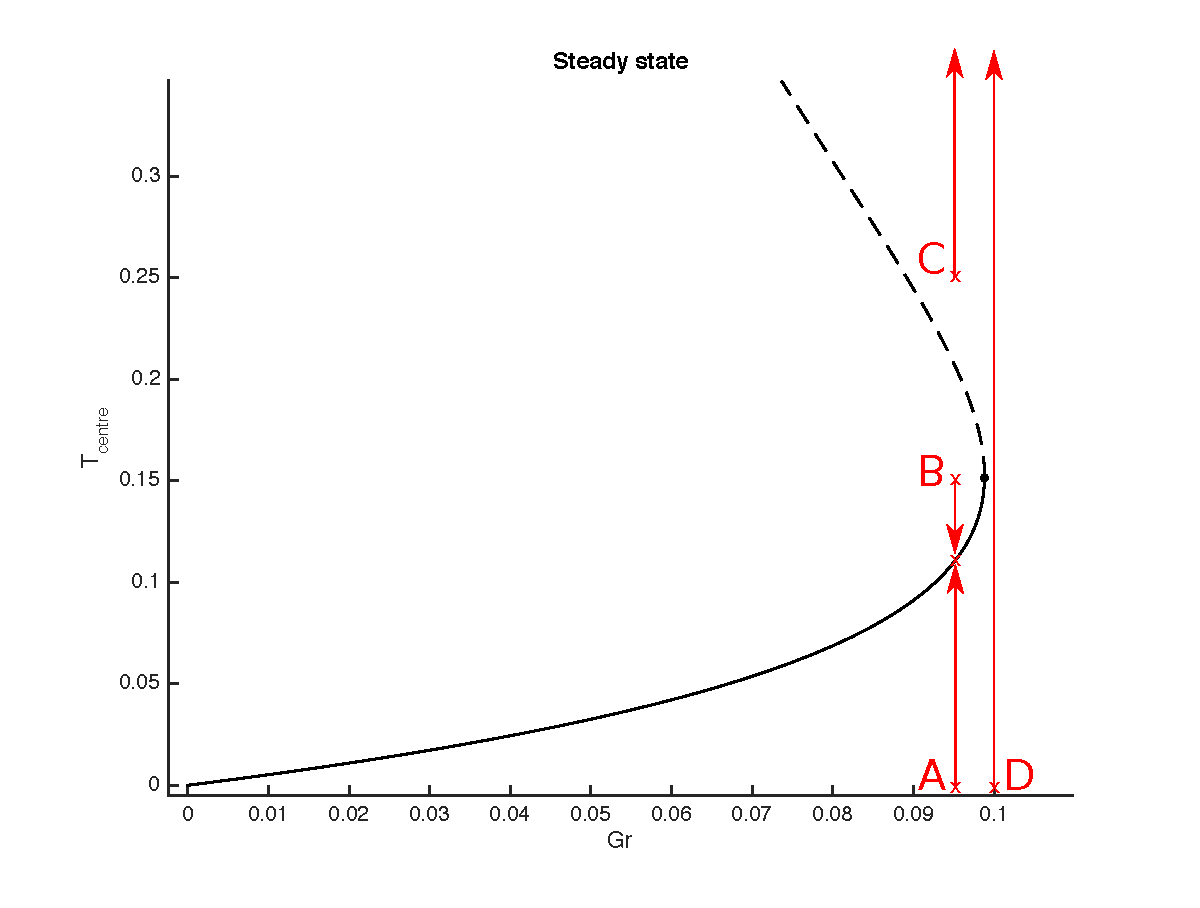
\includegraphics[width=0.32\textwidth]{benchmark_1_T_succombe_0}
  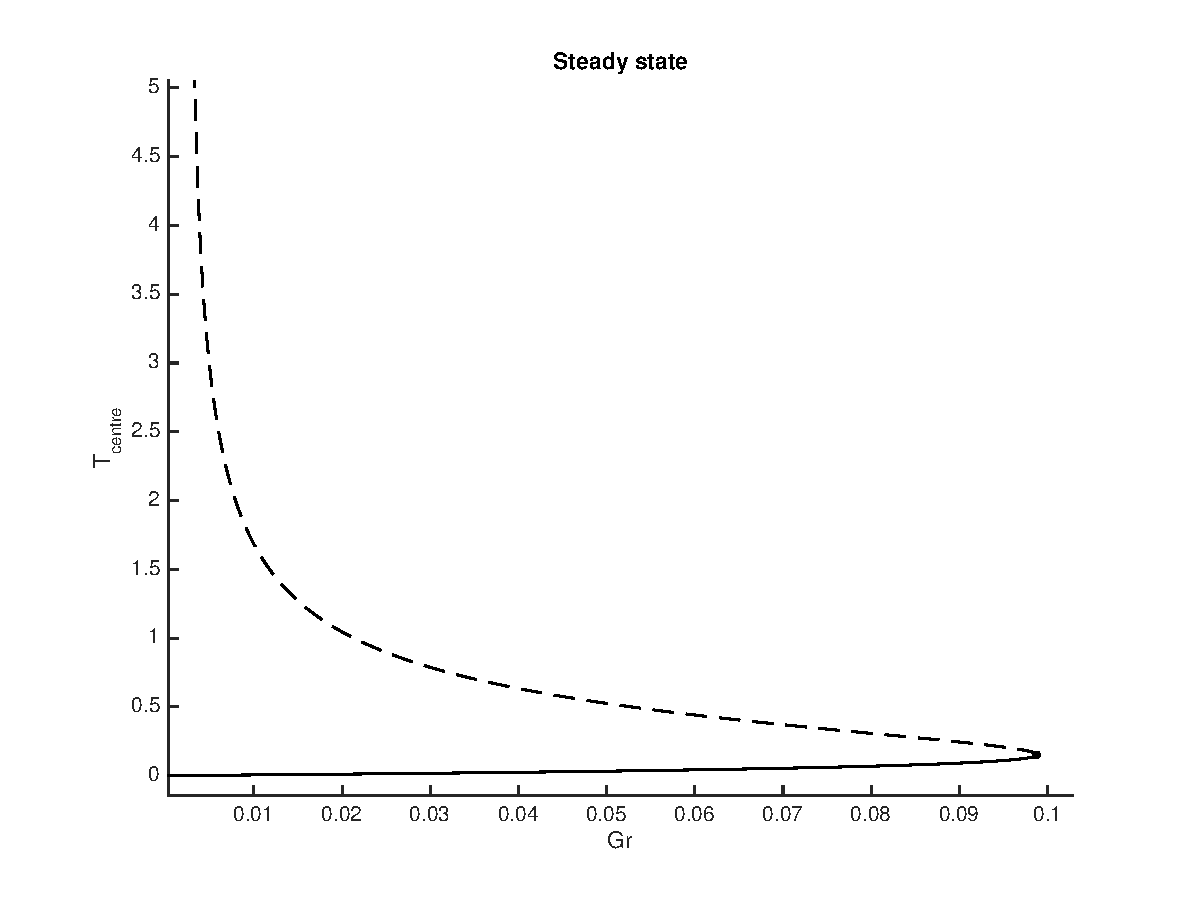
\includegraphics[width=0.32\textwidth]{benchmark_1_T_succombe_1}
  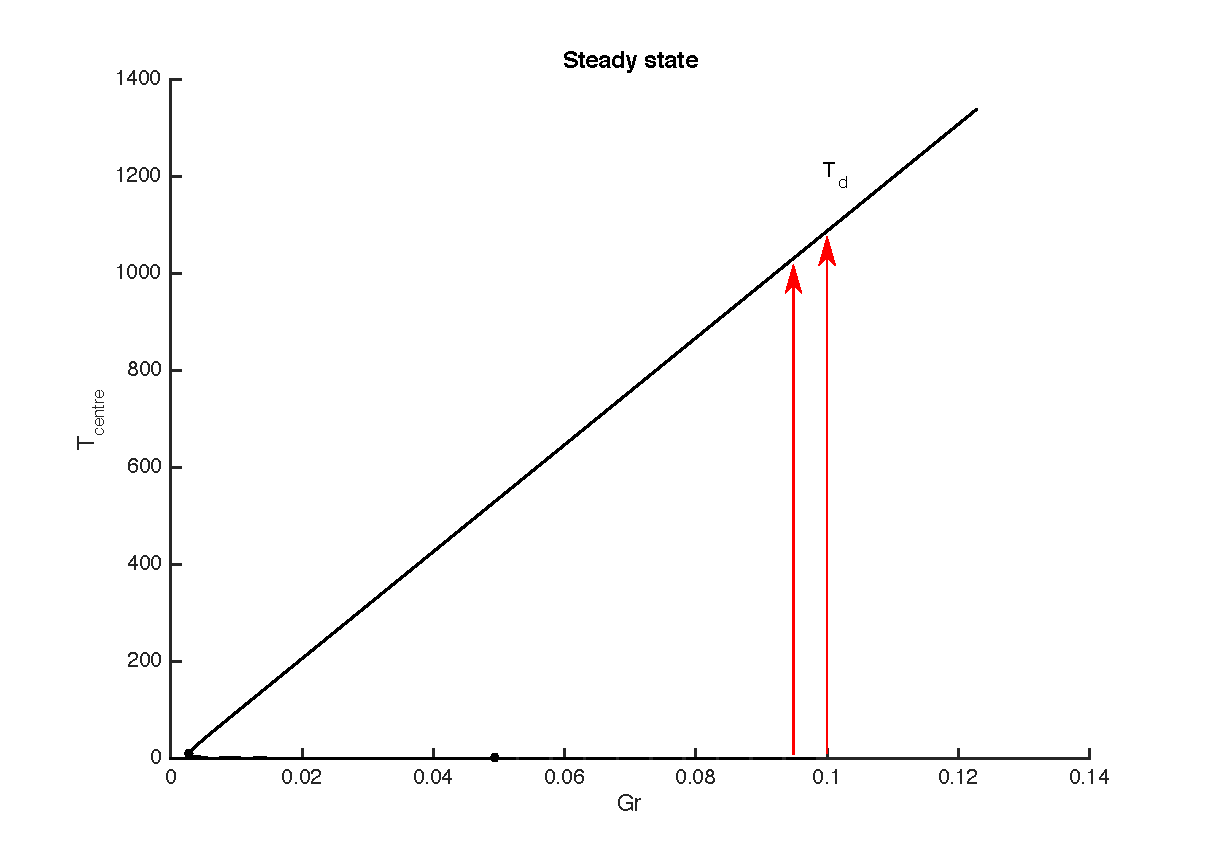
\includegraphics[width=0.32\textwidth]{benchmark_1_T_succombe_2}
  \caption{"S-curve" of the steady state analysis for \texttt{benchmark\_1\_T} with a) zoom on low values of temperatures, showing the four starting conditions and their expected time evolution, b) zoomed out view of the unsteady branch of the "S-curve" in dashed line, and c) even more zoomed out view for larger values of temperatures, showing the higher steady branch where benchmarks C and D converge.}
  \label{fig:benchmark_1_T_succombe}
\end{figure}

This problem is then solved using \moose{} on a generated 1D mesh from -1 to 1 for different values of $Gr$ and the initial solution of the temperature $T_0$ in the center:
\begin{itemize}
\item $Gr=0.095$ and $T_0=0$. In this case, the system should converge increasingly to a centre temperature $T_a\approx0.109$. This case is treated with the input file \texttt{bench1\_a.i} 
\item $Gr=0.095$ and $T_0=0.15$. In this case, the system should converge decreasingly to the same centre temperature $T_b=T_a\approx0.109$. This case is treated with the input file \texttt{bench1\_b.i} 
\item $Gr=0.095$ and $T_0=0.25$. In this case, the system should converge increasingly to a large temperature $T_c>1000$. This case is treated with the input file \texttt{bench1\_c.i} 
\item $Gr=0.1$ and $T_0=0$. In this case, the system should converge increasingly to an even larger temperature $T_d>T_c>1000$. This case is treated with the input file \texttt{bench1\_d.i} 
\end{itemize}

\begin{figure}
  \centering
  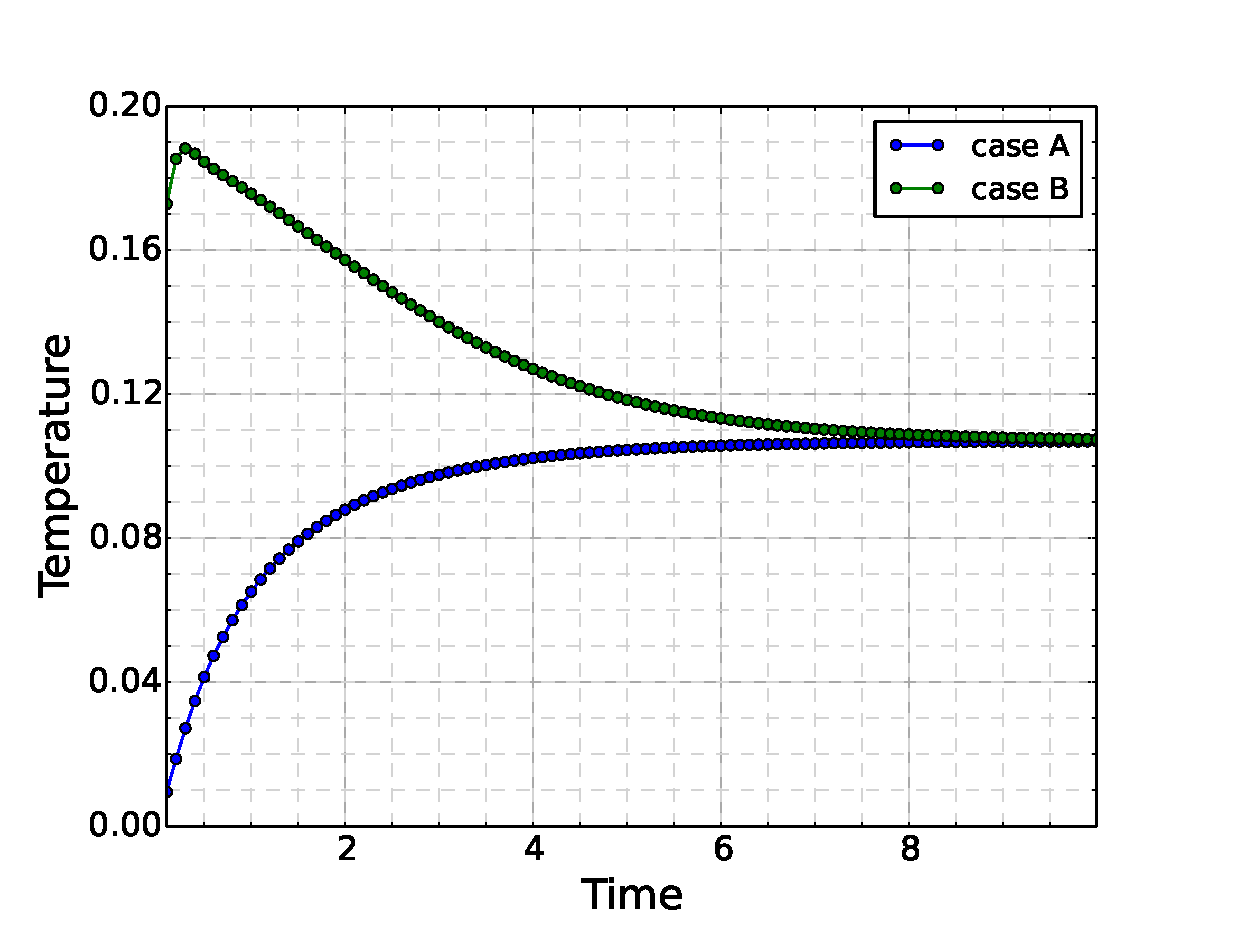
\includegraphics[width=0.48\textwidth]{benchmark_1_T_results_A_B.eps}
  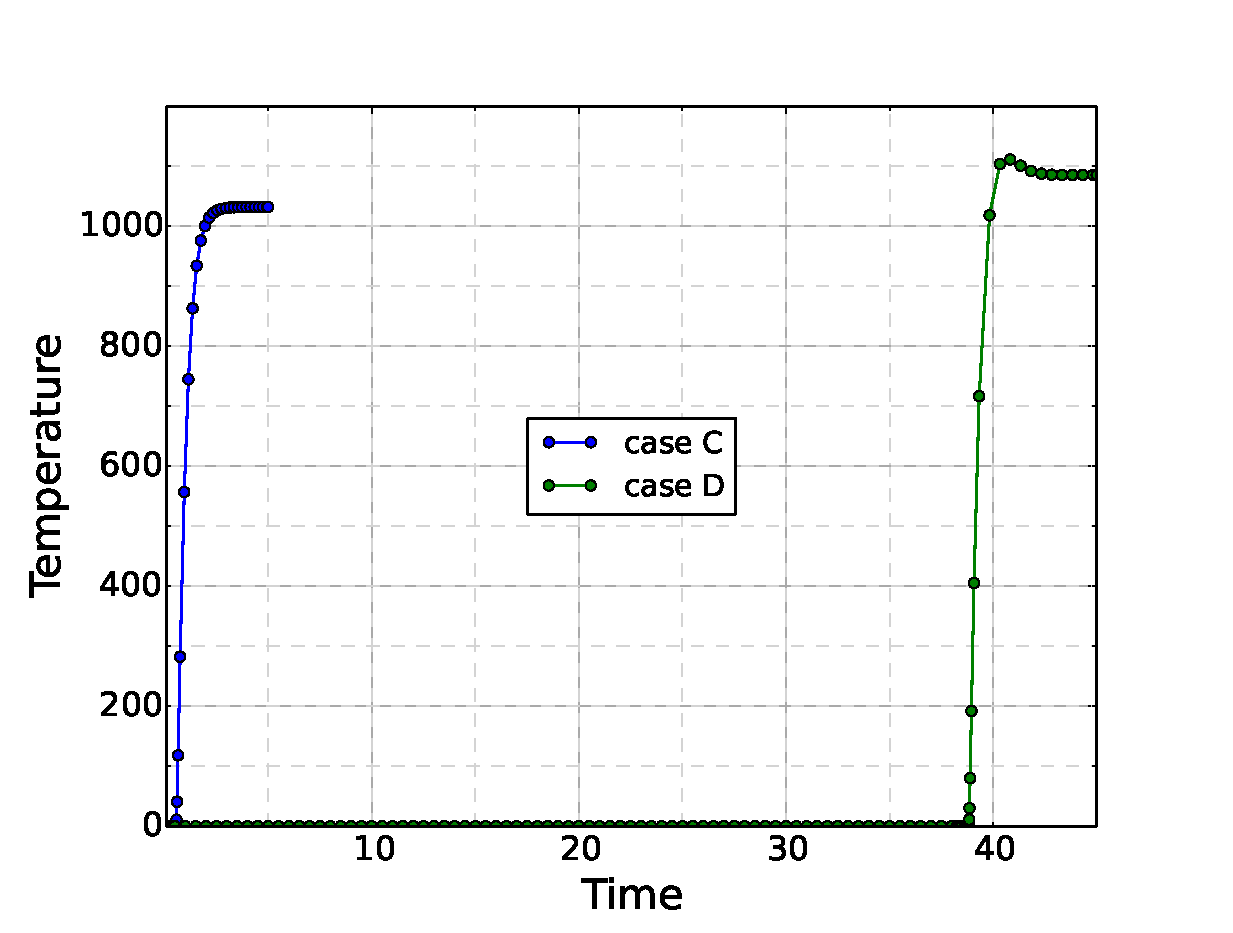
\includegraphics[width=0.48\textwidth]{benchmark_1_T_results_C_D.eps}
  \caption{Time evolution of the numerical results for the four benchmarks: a) cases A and B converge to the lower stable branch (see Fig.~\ref{fig:benchmark_1_T_succombe}), while b) cases C and D converge to the upper stable branch.}
  \label{fig:benchmark_1_T_results}
\end{figure}

The numerical results match the theory with the time evolutions shown on Fig.~\ref{fig:benchmark_1_T_results}.




\appendix

\chapter{Derivations}
\label{chapter:derivations}
This chapter documents some of the derivations used to obtain the equations presented in Sec.\ref{chapter:gov_eqs}.

\section{Mass balance}
\label{sec:mass_balance}
We define the following densities
\begin{subequations}
  \label{eq:rho_1_rho_2}
  \begin{align}
    \rho_1 &= (1-\phi)\rho_s \\
    \rho_2 &= \phi \: \rho_f  
  \end{align}
\end{subequations}

and we use the usual material derivative definition
\begin{equation}
  \label{eq:material_derivative}
  \frac{D^{(i)}.}{D t} = \frac{\partial.}{\partial t} + v^{(i)}_k \frac{\partial.}{\partial x_k}
\end{equation}


\underline{Mass balance for the fluid phase}
\begin{equation}
  \label{eq:fluid_mass_balance_1}
  \frac{\partial \rho_2}{\partial t} + \frac{\partial( \rho_2 V^{(2)}_k)}{\partial x_k}= j_1
\end{equation}

Using Eq.~\ref{eq:rho_1_rho_2}b in Eq.~\ref{eq:fluid_mass_balance_1} we get
\begin{equation}
  \label{eq:fluid_mass_balance_2}
  \phi \frac{\partial \rho_f }{\partial t} + \rho_f\frac{\partial \phi }{\partial t} + \rho_f\frac{\partial( \phi V^{(2)}_k)}{\partial x_k}+ \phi V^{(2)}_k\frac{\partial\rho_f}{\partial x_k} = j_1
\end{equation}
Dividing by $\rho_f$ we obtain
\begin{equation}
  \label{eq:fluid_mass_balance}
  \frac{\phi}{\rho_f} \frac{D^{(2)} \rho_f }{D t} + \frac{\partial \phi }{\partial t} + \frac{\partial( \phi V^{(2)}_k)}{\partial x_k} = \frac{j_1}{\rho_f}
\end{equation}


\underline{Mass balance for the solid phase}
\begin{equation}
  \label{eq:solid_mass_balance_1}
  \frac{\partial \rho_1}{\partial t} + \frac{\partial( \rho_1 V^{(1)}_k)}{\partial x_k}= -j_1
\end{equation}
Using Eq.~\ref{eq:rho_1_rho_2}a in Eq.~\ref{eq:solid_mass_balance_1} we get
\begin{equation}
  \label{eq:solid_mass_balance_2}
  (1-\phi) \frac{\partial \rho_s }{\partial t} - \rho_s\frac{\partial \phi }{\partial t} + \rho_s\frac{\partial( (1-\phi) V^{(1)}_k)}{\partial x_k}+ (1-\phi) V^{(1)}_k\frac{\partial\rho_s}{\partial x_k} = -j_1
\end{equation}
Dividing by $\rho_s$ we obtain
\begin{equation}
  \label{eq:solid_mass_balance}
  \frac{(1-\phi)}{\rho_s} \frac{D^{(1)} \rho_s }{D t} - \frac{\partial \phi }{\partial t} + \frac{\partial(V^{(1)}_k)}{\partial x_k} - \frac{\partial( \phi V^{(1)}_k)}{\partial x_k} = -\frac{j_1}{\rho_s}
\end{equation}

\underline{Mass balance for the mixture (solid + fluid)}

Adding Eq.~\ref{eq:fluid_mass_balance} and Eq.~\ref{eq:solid_mass_balance} gives the mixture mass balance:
\begin{equation}
  \label{eq:mixture_mass_balance}
  \frac{(1-\phi)}{\rho_s} \frac{D^{(1)} \rho_s }{D t} +\frac{\phi}{\rho_f} \frac{D^{(2)} \rho_f }{D t} + \frac{\partial( \phi (V^{(2)}_k -V^{(1)}_k))}{\partial x_k}+ \frac{\partial(V^{(1)}_k)}{\partial x_k}  = \left(\frac{1}{\rho_f} - \frac{1}{\rho_s}\right)j_1
\end{equation}

\underline{Equation of state (EOS)}

\begin{equation}
  \label{eq:density_derivative}
  \frac{d\rho_{(i)}}{\rho_{(i)}} = \left( \frac{d\rho_{(i)}}{dp_f} \right)_T \frac{dp_f}{\rho_{(i)}} +\left( \frac{d\rho_{(i)}}{dT} \right)_p \frac{dT}{\rho_{(i)}}, \:\:\:i\in \{s,f\} 
\end{equation}

Using the definition for compressibility $\beta_{(i)}=\frac{1}{\rho_{(i)}}\left( \frac{d\rho_{(i)}}{dp_f} \right)_T$ and thermal expansion $\lambda_{(i)}=-\frac{1}{\rho_{(i)}}\left( \frac{d\rho_{(i)}}{dT} \right)_{p_f}$ we get the Equation of State (EOS)

\begin{equation}
  \label{eq:eos_def}
  \frac{d\rho_{(i)}}{\rho_{(i)}} = \beta_{(i)} dp_f - \lambda_{(i)} dT, \:\:\:i\in \{s,f\} 
\end{equation}

Using Eq.~\ref{eq:eos_def} in Eq.~\ref{eq:mixture_mass_balance} leads to
\begin{multline}
  \label{eq:mixture_mass_balance2}
  (1-\phi) \left[ \beta_s \frac{D^{(1)}p_f}{Dt} - \lambda_s\frac{D^{(1)}T}{Dt}  \right] + \phi \left[ \beta_f \frac{D^{(2)}p_f}{Dt} - \lambda_f\frac{D^{(2)}T}{Dt}  \right] \\
  + \frac{\partial( \phi (V^{(2)}_k -V^{(1)}_k))}{\partial x_k}+ \frac{\partial(V^{(1)}_k)}{\partial x_k}  = \left(\frac{1}{\rho_f} - \frac{1}{\rho_s}\right)j_1
\end{multline}
Rearranging the terms we get
\begin{multline}
  \label{eq:mixture_mass_balance3}
  \overbrace{\left[(1-\phi)\beta_s + \phi\beta_f\right]}^{\beta_m}  \frac{\partial p_f}{\partial t} 
  - \overbrace{\left[(1-\phi)\lambda_s + \phi\lambda_f\right]}^{\lambda_m} \frac{\partial T}{\partial t} \\
  + \left[(1-\phi)\beta_s V^{(1)}_k + \phi\beta_f V^{(2)}_k \right] \frac{\partial p_f}{\partial x_k} 
  - \left[(1-\phi)\lambda_s V^{(1)}_k + \phi\lambda_f V^{(2)}_k \right] \frac{\partial T}{\partial x_k} \\
  + \frac{\partial( \phi (V^{(2)}_k -V^{(1)}_k))}{\partial x_k}+ \frac{\partial(V^{(1)}_k)}{\partial x_k}  = \left(\frac{1}{\rho_f} - \frac{1}{\rho_s}\right)j_1
\end{multline}

\underline{Normalisation}

In order to deal with dimensionless parameters we introduce the following normalised variables
\begin{subequations}
  \label{eq:def_normalisations}
  \begin{align}
  p^* &= \frac{p_f}{\sigma_{ref}}, \\   
  T^* &= \frac{T-T_{ref}}{\delta T_{ref}}, \\   
  x^* &= \frac{x}{x_{ref}}, \\   
  t^* &= \frac{c_{th}}{x^2_{ref}}t, \\   
  V^* &= \frac{V}{V_{ref}}.
  \end{align}
\end{subequations}

Dividing Eq.~\ref{eq:mixture_mass_balance3} by $\beta_m$ and switching to the normalised variables we get

\begin{multline}
  \label{eq:mixture_mass_balance4}
  \frac{\sigma_{ref} \: c_{th}}{x^2_{ref}} \frac{\partial p^*}{\partial t^*} 
  - \frac{\lambda_m \: \delta \: T_{ref} \: c_{th}}{\beta_m\:x^2_{ref}} \frac{\partial T^*}{\partial t^*} \\
  + \frac{V_{ref} \: \sigma_{ref}}{x_{ref}}\left[\frac{(1-\phi)\beta_s V^{*(1)}_k + \phi\beta_f V^{*(2)}_k}{\beta_m} \right] \frac{\partial p^*}{\partial x^*_k} \\
  - \frac{V_{ref}\:\delta\:T_{ref}}{x_{ref}}\left[\frac{(1-\phi)\lambda_s V^{*(1)}_k + \phi\lambda_f V^{*(2)}_k}{\beta_m} \right] \frac{\partial T*}{\partial x^*_k} \\
  + \frac{V_{ref}}{\beta_m\:x_{ref}} \frac{\partial( \phi (V^{*(2)}_k -V^{*(1)}_k))}{\partial x^*_k}
  + \frac{V_{ref}}{\beta_m\:x_{ref}} \frac{\partial(V^{*(1)}_k)}{\partial x^*_k}  
  = \frac{1}{\beta_m} \left(\frac{1}{\rho_f} - \frac{1}{\rho_s}\right)j_1
\end{multline}

This can be rewritten as

\begin{multline}
  \label{eq:mixture_mass_balance5}
  \frac{\partial p^*}{\partial t^*} 
  - \overbrace{\frac{\lambda_m \: \delta \: T_{ref}}{\beta_m\:\sigma_{ref}}}^{\Lambda} \frac{\partial T^*}{\partial t^*} 
  + \overbrace{\frac{x_{ref}\:V_{ref}}{c_{th}}}^{Pe}  \overbrace{\left[\frac{(1-\phi)(\sigma_{ref}\beta_s) V^{*(1)}_k + \phi(\sigma_{ref}\beta_f) V^{*(2)}_k}{\sigma_{ref}\beta_m} \right]}^{\vec{v}^p} \frac{\partial p^*}{\partial x^*_k} \\
  - \overbrace{\frac{x_{ref}\:V_{ref}}{c_{th}}}^{Pe} \overbrace{\left[\frac{(1-\phi)(\delta\:T_{ref}\lambda_s) V^{*(1)}_k + \phi(\delta\:T_{ref}\lambda_f) V^{*(2)}_k}{\sigma_{ref}\beta_m} \right]}^{\vec{v}^T} \frac{\partial T*}{\partial x^*_k} \\
  + \frac{x_{ref}\:V_{ref}}{c_{th}\:\beta_m\:\sigma_{ref}}  \frac{\partial}{\partial x^*_k} \underbrace{\left[ \phi (V^{*(2)}_k -V^{*(1)}_k)\right]}_{\text{norm. filtration vec.}} 
  + \underbrace{\frac{x_{ref}\:V_{ref}}{c_{th}}}_{Pe} \frac{1}{\beta_m\:\sigma_{ref}} \underbrace{\frac{\partial(V^{*(1)}_k)}{\partial x^*_k}}_{\dot{\epsilon}^*_V}  \\
  = \frac{x^2_{ref}}{\beta_m\:\sigma_{ref}\:c_{th}} \left(\frac{1}{\rho_f} - \frac{1}{\rho_s}\right)j_1
\end{multline}

with

\begin{subequations}
  \label{eq:def_parameters}
  \begin{align}
  \Lambda &= \frac{\lambda_m \: \delta \: T_{ref}}{\beta_m\:\sigma_{ref}}=\frac{\lambda^*_m}{\beta^*_m}, \\   
  \lambda^*_i &= \delta \: T_{ref} \:\lambda_i, \:\:\: i\in\{s,f,m\}\\
  \beta^*_i &= \beta \: \sigma_{ref}, \:\:\: i\in\{s,f,m\}\\
  Pe &= \frac{x_{ref}\:V_{ref}}{c_{th}}, \\   
  v^p &= \frac{(1-\phi)\beta^*_s V^{*(1)}_k + \phi\beta^*_f V^{*(2)}_k}{\beta^*_m}, \\   
  v^T &= \frac{(1-\phi)\lambda^*_s V^{*(1)}_k + \phi\lambda^*_f V^{*(2)}_k}{\beta^*_m}.
  \end{align}
\end{subequations}

The filtration vector $\phi(V^{(2)}_k -V^{(1)}_k)$ can be expressed using Darcy's law as
\begin{equation}
  \label{eq:darcy}
  \phi(V^{(2)}_k -V^{(1)}_k) = -\frac{k}{\mu_f} \left(\frac{\partial p_f}{\partial x_k} - \rho_f\:g\:\vec{e}_z \right)
\end{equation}

In its normalised form it becomes 
\begin{equation}
  \label{eq:darcy_normalised}
  \phi(V^{*(2)}_k -V^{*(1)}_k)
  = -\frac{k}{\mu_f} \frac{\sigma_{ref}}{x_{ref}\:V_{ref}}\left(\frac{\partial p^*}{\partial x^*_k} - \frac{x_{ref}}{\sigma_{ref}}\rho_f\:g\:\vec{e}_z \right)
\end{equation}

The mass balance equation then becomes
\begin{multline}
  \label{eq:mixture_mass_balance6}
  \frac{\partial p^*}{\partial t^*} 
  - \Lambda \frac{\partial T^*}{\partial t^*} 
  + Pe \:\vec{v}^p \frac{\partial p^*}{\partial x^*_k} 
  - Pe \:\vec{v}^T \frac{\partial T*}{\partial x^*_k} \\
  + \frac{\partial}{\partial x^*_k} \left[ \underbrace{\frac{k \: \sigma_{ref}}{\mu_f\:c_{th}\:\beta^*_m}}_{1/Le} \left( \frac{\partial p^*}{\partial x^*_k} - \underbrace{\rho_f \frac{x_{ref}}{\sigma_{ref}}g}_{(\rho_f\:g)^*}\: \vec{e}_z  \right) \right]
  + \frac{Pe}{\beta_m\:\sigma_{ref}} \dot{\epsilon}^*_V  
  = \frac{x^2_{ref}}{\beta_m\:\sigma_{ref}\:c_{th}} \left(\frac{1}{\rho_f} - \frac{1}{\rho_s}\right)j_1
\end{multline}

with the Lewis number defined as $Le = \frac{\mu_f\:c_{th}\:\beta^*_m}{k \: \sigma_{ref}}$ and the normalised gravity term $(\rho_f\:g)^*=\rho_f \frac{x_{ref}}{\sigma_{ref}}g$.

Following \citep[][appendix A]{Alevizos2014}
$j_1 = \omega_F.M_B$, $\omega_F=\frac{\rho_1}{M_{AB}}k_F exp{-Q_F/RT}$ and $\rho_1=(1-\phi)(1-s)\rho_{AB}$, so the volumetric source term $j1$ can be written as
\begin{equation}
  \label{eq:j1_a}
  j_1 =\rho_{AB}\frac{M_B}{M_{AB}}(1-\phi)(1-s) k_F exp{(-Q_F/RT)}
\end{equation}
The RHS term of Eq.~\ref{eq:mixture_mass_balance6} can then be written as
\begin{multline}
  \label{eq:mixture_mass_balance_rhs}
  \frac{x^2_{ref}}{\beta_m\:\sigma_{ref}\:c_{th}} \left(\frac{1}{\rho_f} - \frac{1}{\rho_s}\right)j_1 = \frac{x^2_{ref}}{\beta_m\:\sigma_{ref}\:c_{th}} \left(\frac{1}{\rho_f} - \frac{1}{\rho_s}\right)\rho_{AB}\frac{M_B}{M_{AB}}(1-\phi)(1-s) k_F exp{(-Q_F/RT)} \\
  = \underbrace{\frac{x^2_{ref}k_F }{\beta_m\:\sigma_{ref}\:c_{th}} \frac{\rho_{AB}}{\rho_B}\frac{M_B}{M_{AB}}\left(\frac{\rho_B}{\rho_f} - \frac{\rho_B}{\rho_s}\right)e^{-Ar_F}}_{1/Le_{chem}} \underbrace{(1-\phi)(1-s) \exp{\left( \frac{Ar_F \:\delta T^*}{1+\delta T^*} \right)}}_{\omega^*_F }
\end{multline}

We then arrive to the full mass balance equation Eq.~\ref{eq:final_system_of_equations_dimensionless}b

\section{Energy balance}
\label{sec:energy_balance}
The local form of the energy balance equation reads as follows:
\begin{equation}
  \label{eq:energy_balance}
  (\rho C_p)_m \frac{D^{(m)}T}{Dt} = \kappa \nabla^2 T + \chi \sigma_{ij}.\dot{\epsilon}^{p}_{ij} - \Delta H (\omega_F - \omega_R)
\end{equation}
with $\chi$ the Taylor-Quinney coefficient and $\Delta H=\Delta E=E_F-E_R$ the reaction's specific enthalpy.
The definitions of the reaction rates $\omega_F$ and $\omega_R$ are (from Eq.~\ref{eq:reaction_rate_total})
\begin{subequations}
 \label{eq:reaction_rates}
 \begin{align}
 \omega_F &= k_F (1 - s)(1 - \phi)\frac{\rho_{AB}}{M_{AB}}  e^{-Q_F/RT} \\
 \omega_R &= k_R \:s  (1 - \phi)  \Delta \phi_{chem} \frac{\rho_{A} \rho_{B}}{\rho_{AB}} \frac{M_{AB}}{M_A M_B}  e^{-Q_R/RT}
  \end{align}
\end{subequations}

Using the normalised variable we get
\begin{multline}
  \label{eq:energy_balance1}
  \frac{\delta T_{ref}\:c_{th}}{x^2_{ref}}(\rho C_p)_m \frac{\partial T^*}{\partial t^*} + \frac{\delta T_{ref}\:v_{ref}}{x_{ref}}(\rho C_p)_m \:\bar{v}.\frac{\partial T^*}{\partial x^*} \\ 
  - \frac{\kappa\:\delta T_{ref}}{x^2_{ref}} \nabla^2 T - \frac{\sigma_{ref}\:c_{th}}{x^2_{ref}} \chi \sigma^*_{ij}.\dot{\epsilon}^{*(p)}_{ij} \\
  - \Delta H.k_F (1 - s)(1 - \phi)\frac{\rho_{AB}}{M_{AB}}  e^{-Q_F/RT} \\
  + \Delta H. k_R \:s  (1 - \phi)  \Delta \phi_{chem} \frac{\rho_{A} \rho_{B}}{\rho_{AB}} \frac{M_{AB}}{M_A M_B}  e^{-Q_R/RT} = 0
\end{multline}

Note that the reference strain rate is also rescaled so 
\begin{equation}
  \dot{\epsilon}^*_0 = \dot{\epsilon}_0 \frac{x^2_{ref}}{c_{th}}
\end{equation}

This leads to 
\begin{multline}
  \label{eq:energy_balance2}
  \frac{\partial T^*}{\partial t^*} + \overbrace{\frac{x_{ref}\:v_{ref}}{c_{th}}}^{Pe}\:\bar{v}.\frac{\partial T^*}{\partial x^*} - \overbrace{\frac{\kappa}{(\rho C_p)_m}}^{c_{th}}\frac{1}{c_{th}} \nabla^2 T - \overbrace{\frac{\sigma_{ref}}{\delta T_{ref}(\rho C_p)_m} \chi}^{Gr} \sigma^*_{ij}.\dot{\epsilon}^{*(p)}_{ij} \\
  - \underbrace{\frac{\Delta H\:x^2_{ref} k_F }{\delta T_{ref}\:\kappa}\frac{\rho_{AB}}{M_{AB}}e^{-Ar_F}}_{Da_{endo}} (1 - s)(1 - \phi)e^{\frac{Ar_F\:\delta T^*}{1+\delta T^*}} \\
   + \underbrace{\frac{\Delta H x^2_{ref} k_R}{\delta T_{ref}\kappa} \frac{\rho_{A} \rho_{B}}{\rho_{AB}} \frac{M_{AB}}{M_A M_B} e^{-Ar_R}}_{Da_{exo}}\:s  (1 - \phi)\Delta \phi_{chem} e^{\frac{Ar_R\:\delta T^*}{1+\delta T^*}}= 0
\end{multline}
and finally to Eq.~\ref{eq:final_system_of_equations_dimensionless}c

\section{Jacobians}
Numerical convergence can be helped by providing the jacobians and off-diagonal terms for the kernel residuals, even though \moose{} does not explicitly require them. It is a trial-and-error process to check if the improvement in convergence justifies the cost of computing those terms. See the \moose{} workshop manual on \url{http://mooseframework.org/documentation/} for more details.


%\mathscr{R}
If $R(u)$ is the residual for the variable $u$, the jacobian matrix $J$ is defined as
\begin{equation}
  \label{eq:def_jacobian}
  J_{ij}(u) = \frac{\partial R_i(u)}{\partial u_j}
\end{equation}
and the off-diagonal jacobian term for another coupled variable $v$ as
\begin{equation}
  \label{eq:def_off_diag_jacobian}
  J^{(\text{off diag})}_{ij}(u) = \frac{\partial R_i(u)}{\partial v_j}
\end{equation}

\subsection{RedbackMassConvection}
The residual is defined as
\begin{equation}
  R = Pe\: v^p.\nabla p^* - Pe\:v^T.\nabla T^*
\end{equation}
with (see Eq.\ref{eq:final_system_of_equations_dimensionless})
\begin{align*}
  v_i^p &= (1-\phi)\frac{\beta^*_s}{\beta^*_m} v_i^{*(s)} + 
    \phi\frac{\beta^*_f}{\beta^*_m}v_i^{*(f)}, \\
  v^T_i &= (1-\phi)\frac{\lambda^*_s}{\beta^*_m} v_i^{*(s)} + 
    \phi\frac{\lambda^*_f}{\beta^*_m} v_i^{*(f)}.
\end{align*}
Noting that $\frac{\partial \nabla u}{\partial u_j}=\nabla \phi_j$ for any variable $u$ (see \moose{} documentation),
\begin{equation}
  \label{eq:def_jac_mass_conv}
  J = \frac{\partial R}{\partial p^*} = Pe \frac{\partial v^p}{\partial p^*}.\nabla p^* + Pe\:v^p\:\nabla \phi_j - Pe\frac{\partial v^T}{\partial p^*}.\nabla T^*
\end{equation}
The normalised filtration vector (Eq.~\ref{eq:darcy_normalised}) can be rewritten as
\begin{equation}
 \label{eq:darcy_normalised2}
  \phi (v^{*(f)} - v^{*(s)}) = -\frac{\beta^*_m}{Le\:Pe} \left(\nabla p^* - \rho_f\:g^* \right)
\end{equation}

Deriving that equation and adding the equation of state (Eq.~\ref{eq:eos_def}) we get
\begin{equation}
  \frac{\partial (\phi v^{*(f)})}{\partial p^*} = -\frac{\beta^*_m}{Le\:Pe} \left(\nabla \phi_j - \beta^*_f\rho_f\:g^* \right)
\end{equation}
under the following simplifying assumptions:
\begin{itemize}
 \item $\frac{\partial v^{(s)}}{\partial p^*}=0$
 \item $\frac{\partial \mu_f}{\partial p^*}=0$
 \item $\frac{\partial \phi}{\partial p^*}=0$
\end{itemize}
Using $\frac{\partial \rho_f}{\partial p^*} = \beta^*_f \: \rho_f$ we get
\begin{subequations}
  \label{eq:derivatives_vT_vp}
  \begin{align}
     \frac{\partial v^p}{\partial p^*} &= -\frac{\beta^*_f}{Le\:Pe} \left(\nabla \phi_j - \beta^*_f\rho_f\:g^* \right) \\
  \frac{\partial v^T}{\partial p^*} &= -\frac{\lambda^*_f}{Le\:Pe} \left(\nabla \phi_j - \beta^*_f\rho_f\:g^* \right)
  \end{align}
\end{subequations}


Eq.~\ref{eq:def_jac_mass_conv} then becomes
\begin{subequations}
  \label{eq:jac_mass_conv1}
  \begin{align}
  J &= Pe \frac{\partial v^p}{\partial p^*}.\nabla p^*
  	+ Pe\:v^p\:\nabla \phi_j - Pe\frac{\partial v^T}{\partial p^*}.\nabla T^* \\ \nonumber
  	&= -\frac{1}{Le} \left(\nabla \phi_j - \beta^*_f\rho_f\:g^* \right) (\beta^*_f\nabla p^* - \lambda^*_f\nabla T^*) + Pe\:v^p\:\nabla \phi_j \\ \nonumber
  	&= \left( Pe\:v^p -\frac{1}{Le}(\beta^*_f\nabla p^* - \lambda^*_f\nabla T^*) \right)\nabla \phi_j + \frac{1}{Le} \beta^*_f\rho_f\:g^*(\beta^*_f\nabla p^* - \lambda^*_f\nabla T^*) \\ \nonumber
  \end{align}
\end{subequations}

Using $\frac{\partial \rho_f}{\partial T^*} = -\lambda^*_f \: \rho_f$ we get
\begin{subequations}
  \begin{align}
  \frac{\partial v^p}{\partial T^*} &= -\frac{\beta^*_f \lambda^*_f}{Le\:Pe} \rho_f\:g^* \\
  \frac{\partial v^T}{\partial T^*} &= -\frac{\lambda^{*2}_f}{Le\:Pe} \rho_f\:g^* \\
  \end{align}
\end{subequations}

The off-diagonal jacobian with respect to temperature is defined as
\begin{subequations}
  \label{eq:off_diag_jac_mass_conv1}
  \begin{align}
  J^T &= \frac{\partial R}{\partial T^*} = Pe \frac{\partial v^p}{\partial T^*}.\nabla p^* - Pe\:\frac{\partial v^T}{\partial T^*}\nabla T* - Pe\:v^T\:\nabla \phi_j \\ \nonumber
    &=  -\frac{\lambda^*_f}{Le} \rho_f\:g^* (\beta^*_f \nabla p^* - \lambda^*_f \nabla T*) - Pe\:v^T\:\nabla \phi_j \\ \nonumber
  \end{align}
\end{subequations}

\subsection{RedbackThermalConvection}
The residual is defined as
\begin{equation}
  R = Pe\: \bar{v}.\nabla T^*
\end{equation}
and the corresponding jacobian as
\begin{equation}
  \label{eq:def_jac_heat_conv}
  J = \frac{\partial R}{\partial T^*} = Pe \frac{\partial \bar{v}}{\partial T^*}.\nabla T^* + Pe\:\bar{v}\:\nabla \phi_j.
\end{equation}

From the definition of the normalised filtration velocity (Eq.~\ref{eq:darcy_normalised2}) we get
\begin{equation}
  \frac{\partial v^{*(f)}}{\partial T^*} = -\frac{\beta^*_m \lambda^*_f}{Le\:Pe\:\phi}\rho_f\:g^*
\end{equation}

From the definition of the mixture barycentric velocity $\bar{v} = \frac{\rho_s}{\bar{\rho}} v^{*(s)} + \frac{\rho_f}{\bar{\rho}} v^{*(f)}$ and following the same assumptions that led to Eq.~\ref{eq:derivatives_vT_vp} we write
\begin{subequations}
  \begin{align}
  \frac{\partial \bar{v}}{\partial T^*} &= -\frac{1}{\bar{\rho}^2}\frac{\partial \bar{\rho}}{\partial T^*} (\rho_s v^{*(s)} + \rho_f v^{*(f)}) + \frac{1}{\bar{\rho}} \left[ \frac{\partial \rho_s}{\partial T^*}v^{*(s)} +\frac{\partial \rho_f}{\partial T^*}v^{*(f)} +\rho_f\frac{\partial v^{*(f)}}{\partial T^*}  \right]\\ \nonumber
  &= -\frac{1}{\bar{\rho}}\frac{\partial \bar{\rho}}{\partial T^*}\bar{v} + \frac{1}{\bar{\rho}} \left[ \frac{\partial \rho_s}{\partial T^*}v^{*(s)} +\frac{\partial \rho_f}{\partial T^*}v^{*(f)} +\rho_f\frac{\partial v^{*(f)}}{\partial T^*}  \right]\\ \nonumber
  &= \frac{1}{\bar{\rho}}\left[(1-\phi)\lambda^{*(s)}\rho_s + \phi\lambda^{*(f)}\rho_s \right]\bar{v} - \frac{1}{\bar{\rho}} \left[ \lambda^{*(s)}\rho_s v^{*(s)} + \lambda^{*(f)}\rho_f v^{*(f)} \right] - \frac{\rho_f}{\bar{\rho}}\frac{\beta^*_m \lambda^*_f}{Le\:Pe\:\phi}\rho_f\:g^*  \\ \nonumber
  &= ... \\ \nonumber
  &= \frac{1}{\bar{\rho}}\left[ \lambda^*_m \rho_s \bar{v} - \lambda^*_s \rho_s v^{*(s)} - \lambda^*_f \rho_f v^{*(f)}    \right] - \frac{\rho_f}{\bar{\rho}}\frac{\beta^*_m \lambda^*_f}{Le\:Pe\:\phi}\rho_f\:g^*  \\ \nonumber
  \end{align}
\end{subequations}

For the off-diagonal term with respect to pore pressure we get
\begin{subequations}
  \begin{align}
  \frac{\partial \bar{v}}{\partial p^*} =& -\frac{1}{\bar{\rho}^2}\frac{\partial \bar{\rho}}{\partial p^*} (\rho_s v^{*(s)} + \rho_f v^{*(f)}) + \frac{1}{\bar{\rho}} \left[ \frac{\partial \rho_s}{\partial p^*}v^{*(s)} +\frac{\partial \rho_f}{\partial p^*}v^{*(f)} +\rho_f\frac{\partial v^{*(f)}}{\partial p^*}  \right]\\ \nonumber
  =& -\frac{1}{\bar{\rho}}\frac{\partial \bar{\rho}}{\partial p^*}\bar{v} + \frac{1}{\bar{\rho}} \left[ \frac{\partial \rho_s}{\partial p^*}v^{*(s)} +\frac{\partial \rho_f}{\partial p^*}v^{*(f)} +\rho_f\frac{\partial v^{*(f)}}{\partial p^*}  \right]\\ \nonumber
  =& -\frac{1}{\bar{\rho}}\left[(1-\phi)\beta^{*(s)}\rho_s + \phi\beta^{*(f)}\rho_s \right]\bar{v} + \frac{1}{\bar{\rho}} \left[ \beta^{*(s)}\rho_s v^{*(s)} + \beta^{*(f)}\rho_f v^{*(f)} \right] \\ \nonumber
  &- \frac{\rho_f}{\bar{\rho}}\frac{\beta^*_m}{Le\:Pe\:\phi} \left(\nabla \phi_j - \beta^*_f\rho_f\:g^* \right)  \\ \nonumber
  =& ... \\ \nonumber
  =& \frac{1}{\bar{\rho}}\left[ -\beta^*_m \rho_s \bar{v} + \beta^*_s \rho_s v^{*(s)} + \beta^*_f \rho_f v^{*(f)}    \right] - \frac{\rho_f}{\bar{\rho}}\frac{\beta^*_m}{Le\:Pe\:\phi} \left(\nabla \phi_j - \beta^*_f\rho_f\:g^* \right)  \\ \nonumber
  \end{align}
\end{subequations}



%\addcontentsline{toc}{chapter}{\numberline{}Bibliography}
%\bibliographystyle{unsrt}
%\begin{thebibliography}{99}
%\bibitem{richards1931}LA Richards ``Capillary conduction of
%  liquids through porous mediums''   Physics 1 (1931) pp 318--333
%\end{thebibliography}

\bibliographystyle{aps-nameyear}      % American Physical Society (APS) style, author-year citations
\bibliography{redback}                % name your BibTeX data base
\nocite{*}

\end{document}

